\documentclass{article}

\usepackage[utf8]{inputenc}
\usepackage{graphicx} 
\usepackage{booktabs} 
\usepackage{hyperref} 
\usepackage{float}
\usepackage{caption}
\usepackage{amsmath}

\title{the Impact of News Information Acquisition and Cognition}
\author{Chuanyi You\\Chuyi Zheng\\Cunyu Zhang\\Zixuan Yang}
\date{\today}

\begin{document}

\maketitle
\tableofcontents
\newpage

\section{Background}

In contemporary society, the proliferation of news and information acquisition channels has had a profound impact on individual social attitudes and cognitive behaviors. The "2019 College Students' Social Mentality Survey," led by Dr. Ma Deyong, a professor of political science at Renmin University of China, is designed to explore how Chinese college students access news and information and the subsequent effect on their perception of societal, political, and economic issues.

This survey spans a comprehensive range of topics, from basic demographic information of respondents, such as age, gender, and educational background, to their satisfaction with the country's political and economic state, and their trust and preference towards various news media channels. It also delves into students' interest in political news, the amount of time they spend on such news, and their views on the challenges faced by media outlets in delivering truthful reporting.

The research based on the survey aims to explore the impact of consuming political news on college students' perceptions and sentiments about the current state of society.

\section{Data}
The data set from the "2019 College Student Information Perception Survey" contains 1,254 entries and 133 columns, indicating a comprehensive set of questions addressed in the survey. 

\subsection{Data Processing}
Within the data set, questions 2 to 9 solicit personal information from respondents, such as age, gender, political affiliation, highest educational qualification, academic institution tier, field of study, family annual income, and hometown location. These variables will serve as control variables in the research. Questions 10, 11, and 12 investigate the respondents' satisfaction levels regarding politics, the economy, and personal life, respectively. These will act as dependent variables to assess the students' cognition. Questions 13, 14, and 15 explore the independent variables of interest for our research question, specifically the college students' interest in political news, the time spent browsing news, and the channels used for news consumption. The news channels variable is further processed into a binary variable indicating whether respondents access foreign media and their websites. Responses with a completion time of less than ten minutes will be excluded from the analysis. Question 31 serves as a mechanism to identify and eliminate responses from participants who do not answer the survey earnestly. The study does not encompass the survey questions such as college students' personal sentiments and their opinions on the news. Age column is also  removed since the respondenta are all college students.
\subsection{Descriptive Data}
\begin{figure}[H]
\centering
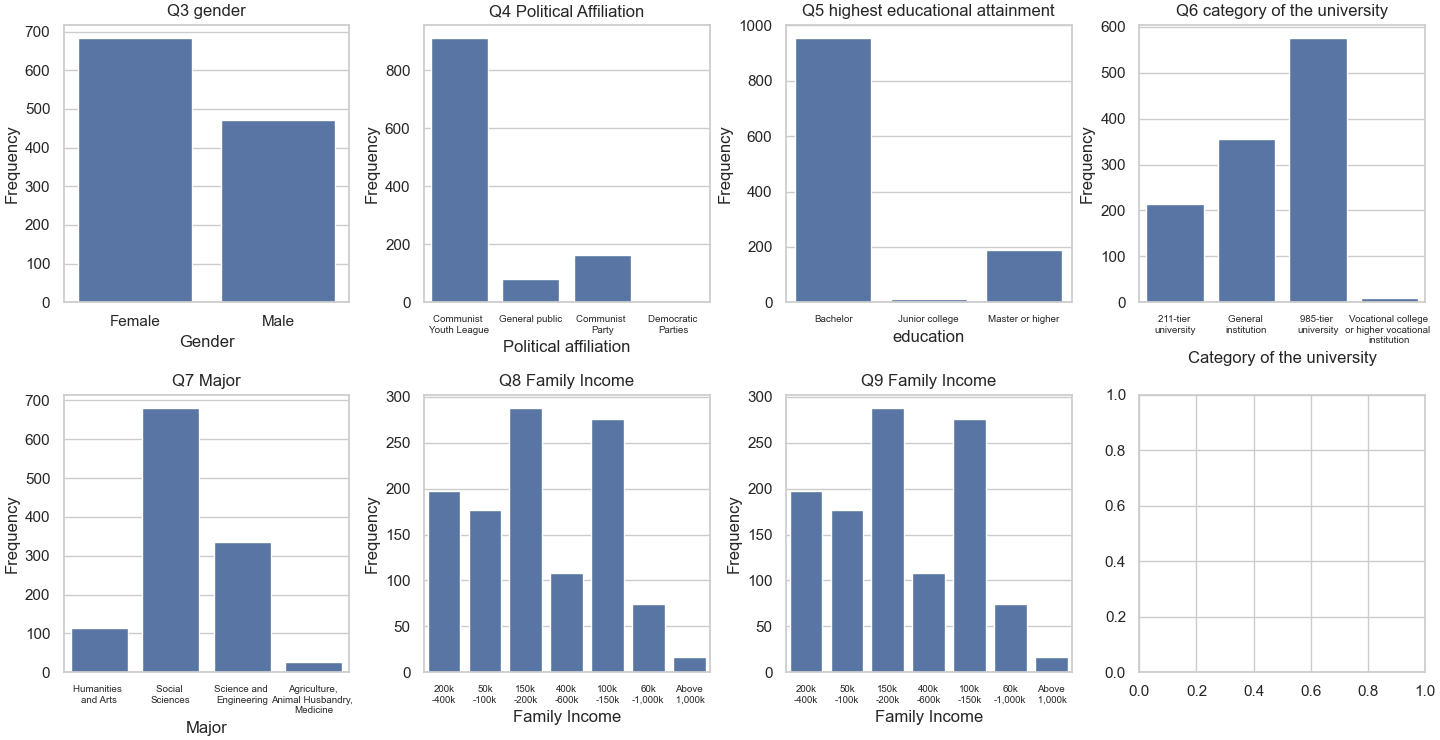
\includegraphics[width=\textwidth]{Figure_1.png}
\caption{Distribution regarding questions 2 to 9, information from respondents, such as age, gender, political affiliation, highest educational qualification, academic institution tier, field of study, family annual income, and hometown location. }
\label{fig:Control Variables}
\end{figure}
In the presented data, the gender distribution shows a slight majority of female respondents over males. Political affiliations lean significantly toward the Communist Youth League, with smaller representations from members of the Communist Party. Educational attainment is predominantly at the bachelor's level, with a smaller proportion holding a master's degree or higher. Considering university categories, the majority of respondents are from 985-tier universities, while vocational colleges account for fewer participants.

The major field of study is led by social sciences, followed by science and engineering. Agriculture, engineering, animal husbandry, and medicine have the smallest numbers of students.

The family income distribution reveals that most respondents come from families earning between 150k to 200k, with fewer in the 100k to 150k bracket. Most respondents are from small towns.


\begin{figure}[H]
\centering
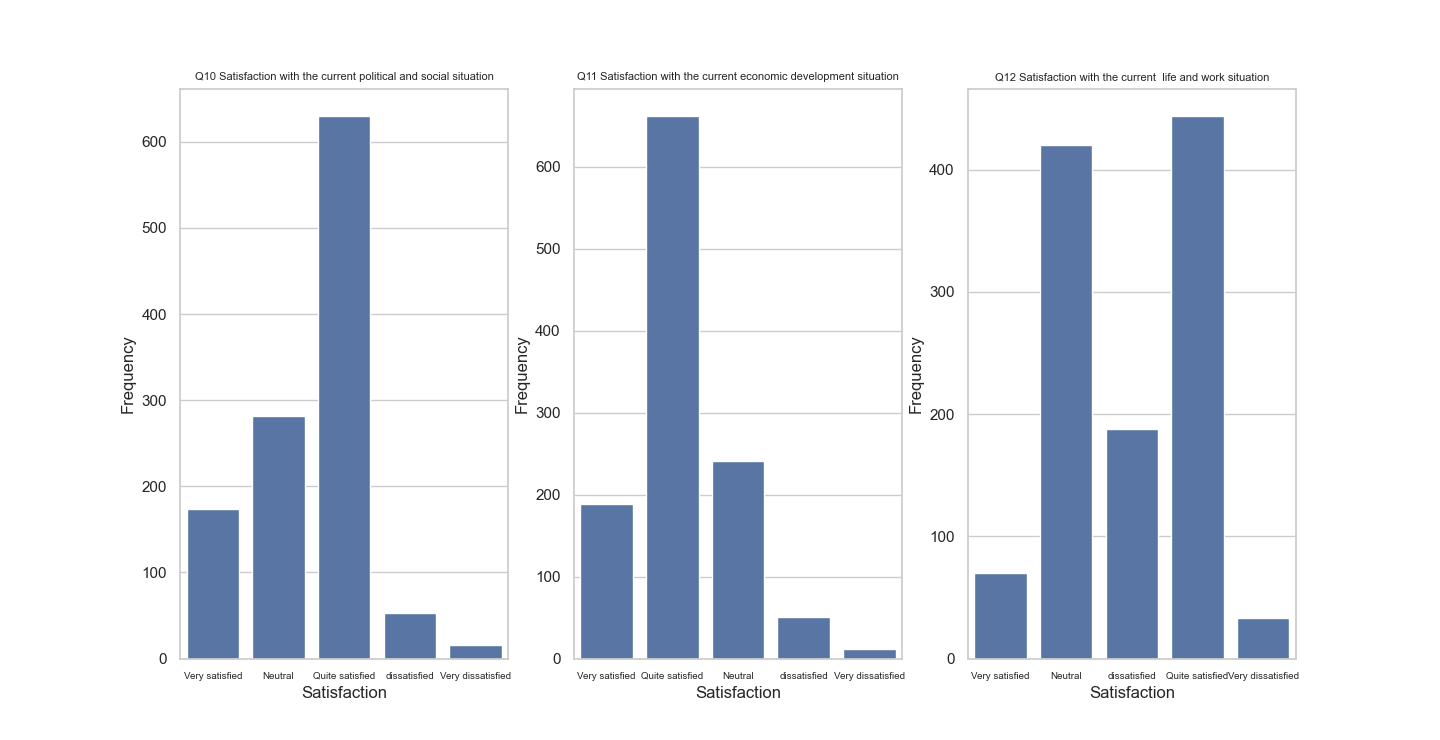
\includegraphics[width=\textwidth]{Figure_2.png}
\caption{Distribution regarding question 10, 11 and 12 investigate the respondents' satisfaction levels regarding politics, the economy, and personal life.}
\label{fig:Dependent variables}
\end{figure}
Satisfaction levels with the current political and social situation, economic development, situations show a trend towards quite satisfied, with a reasonable distribution across the satisfaction spectrum. However, when it comes to personal situation, more people showed their dissatisfaction.
\begin{figure}[H]
\centering
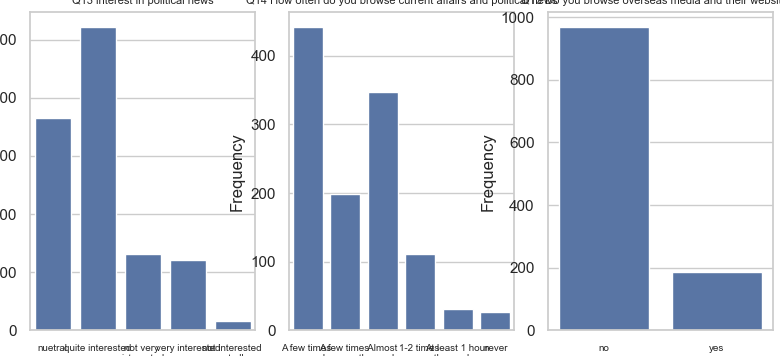
\includegraphics[width=\textwidth]{Figure_3.png}
\caption{Distribution regarding question 12, 13 and 14 investigate the respondents' interest in political news, the time spent browsing news, and the channels used for news consumption}
\label{fig:independent variables}
\end{figure}
Interest in political news is predominantly quite interested to neutral, with very few indicating extreme disinterest. The frequency of browsing current affairs and political news is highest for a few times per week, followed by almost everyday. Finally, the majority of respondents do not browse overseas media and their websites.
\section{Hypothesis}



\subsection{Regression}
\begin{equation}
\begin{aligned}
\text{pol\_sat} &= \beta_0 + \beta_1 \cdot \text{interest} + \beta_2 \cdot \text{time} + \beta_3 \cdot \text{overseas} + \gamma \cdot \text{controls} + \epsilon_1 \nonumber \\
\text{eco\_sati} &= \beta_0 + \beta_1 \cdot \text{interest} + \beta_2 \cdot \text{time} + \beta_3 \cdot \text{overseas} + \gamma \cdot \text{controls} + \epsilon_2 \nonumber \\
\text{lif\_work\_sati} &= \beta_0 + \beta_1 \cdot \text{interest} + \beta_2 \cdot \text{time} + \beta_3 \cdot \text{overseas} + \gamma \cdot \text{controls} + \epsilon_3 \nonumber
\end{aligned}
\end{equation}

\subsection{Robustness}


\section{Results}


\section{Conclusion}


\end{document}